% Created by tikzDevice version 0.11 on 2018-12-11 10:42:22
% !TEX encoding = UTF-8 Unicode
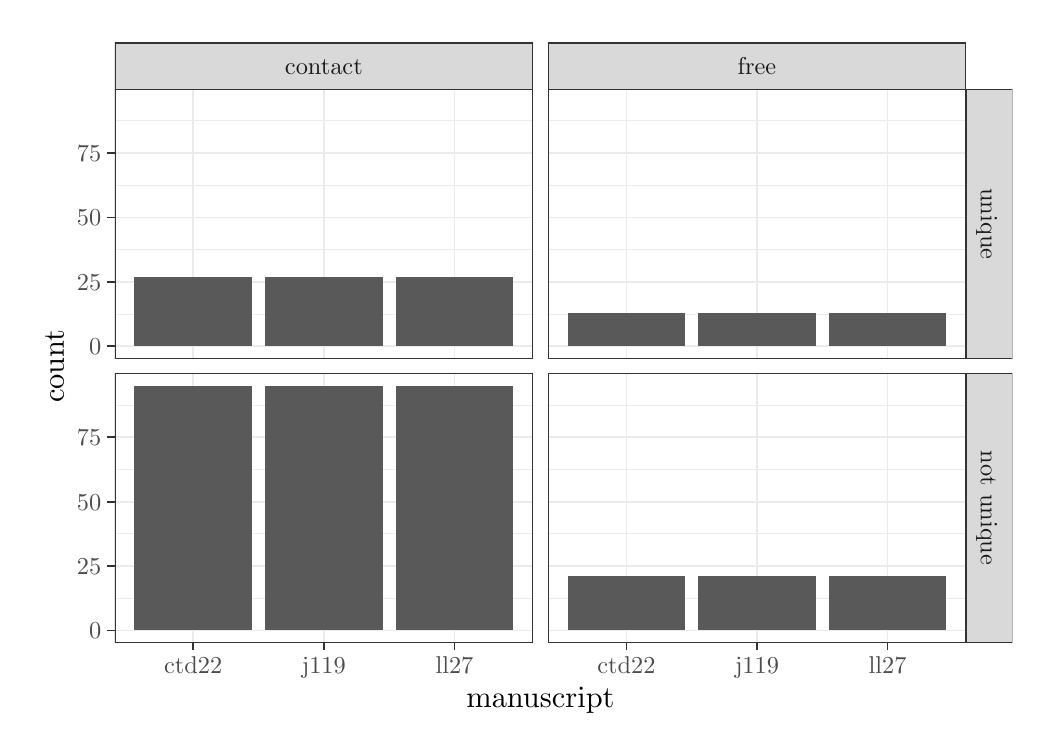
\begin{tikzpicture}[x=1pt,y=1pt]
\definecolor{fillColor}{RGB}{255,255,255}
\path[use as bounding box,fill=fillColor,fill opacity=0.00] (0,0) rectangle (361.35,252.94);
\begin{scope}
\path[clip] (  0.00,  0.00) rectangle (361.35,252.94);
\definecolor{drawColor}{RGB}{255,255,255}
\definecolor{fillColor}{RGB}{255,255,255}

\path[draw=drawColor,line width= 0.6pt,line join=round,line cap=round,fill=fillColor] (  0.00, -0.00) rectangle (361.35,252.94);
\end{scope}
\begin{scope}
\path[clip] ( 31.52,133.43) rectangle (182.53,230.64);
\definecolor{fillColor}{RGB}{255,255,255}

\path[fill=fillColor] ( 31.52,133.43) rectangle (182.53,230.64);
\definecolor{drawColor}{gray}{0.92}

\path[draw=drawColor,line width= 0.3pt,line join=round] ( 31.52,149.48) --
	(182.53,149.48);

\path[draw=drawColor,line width= 0.3pt,line join=round] ( 31.52,172.73) --
	(182.53,172.73);

\path[draw=drawColor,line width= 0.3pt,line join=round] ( 31.52,195.99) --
	(182.53,195.99);

\path[draw=drawColor,line width= 0.3pt,line join=round] ( 31.52,219.25) --
	(182.53,219.25);

\path[draw=drawColor,line width= 0.6pt,line join=round] ( 31.52,137.85) --
	(182.53,137.85);

\path[draw=drawColor,line width= 0.6pt,line join=round] ( 31.52,161.11) --
	(182.53,161.11);

\path[draw=drawColor,line width= 0.6pt,line join=round] ( 31.52,184.36) --
	(182.53,184.36);

\path[draw=drawColor,line width= 0.6pt,line join=round] ( 31.52,207.62) --
	(182.53,207.62);

\path[draw=drawColor,line width= 0.6pt,line join=round] ( 59.83,133.43) --
	( 59.83,230.64);

\path[draw=drawColor,line width= 0.6pt,line join=round] (107.02,133.43) --
	(107.02,230.64);

\path[draw=drawColor,line width= 0.6pt,line join=round] (154.22,133.43) --
	(154.22,230.64);
\definecolor{fillColor}{gray}{0.35}

\path[fill=fillColor] ( 38.60,137.85) rectangle ( 81.07,162.97);

\path[fill=fillColor] ( 85.79,137.85) rectangle (128.26,162.97);

\path[fill=fillColor] (132.98,137.85) rectangle (175.45,162.97);
\definecolor{drawColor}{gray}{0.20}

\path[draw=drawColor,line width= 0.6pt,line join=round,line cap=round] ( 31.52,133.43) rectangle (182.53,230.64);
\end{scope}
\begin{scope}
\path[clip] ( 31.52, 30.72) rectangle (182.53,127.93);
\definecolor{fillColor}{RGB}{255,255,255}

\path[fill=fillColor] ( 31.52, 30.72) rectangle (182.53,127.93);
\definecolor{drawColor}{gray}{0.92}

\path[draw=drawColor,line width= 0.3pt,line join=round] ( 31.52, 46.77) --
	(182.53, 46.77);

\path[draw=drawColor,line width= 0.3pt,line join=round] ( 31.52, 70.03) --
	(182.53, 70.03);

\path[draw=drawColor,line width= 0.3pt,line join=round] ( 31.52, 93.28) --
	(182.53, 93.28);

\path[draw=drawColor,line width= 0.3pt,line join=round] ( 31.52,116.54) --
	(182.53,116.54);

\path[draw=drawColor,line width= 0.6pt,line join=round] ( 31.52, 35.14) --
	(182.53, 35.14);

\path[draw=drawColor,line width= 0.6pt,line join=round] ( 31.52, 58.40) --
	(182.53, 58.40);

\path[draw=drawColor,line width= 0.6pt,line join=round] ( 31.52, 81.65) --
	(182.53, 81.65);

\path[draw=drawColor,line width= 0.6pt,line join=round] ( 31.52,104.91) --
	(182.53,104.91);

\path[draw=drawColor,line width= 0.6pt,line join=round] ( 59.83, 30.72) --
	( 59.83,127.93);

\path[draw=drawColor,line width= 0.6pt,line join=round] (107.02, 30.72) --
	(107.02,127.93);

\path[draw=drawColor,line width= 0.6pt,line join=round] (154.22, 30.72) --
	(154.22,127.93);
\definecolor{fillColor}{gray}{0.35}

\path[fill=fillColor] ( 38.60, 35.14) rectangle ( 81.07,123.51);

\path[fill=fillColor] ( 85.79, 35.14) rectangle (128.26,123.51);

\path[fill=fillColor] (132.98, 35.14) rectangle (175.45,123.51);
\definecolor{drawColor}{gray}{0.20}

\path[draw=drawColor,line width= 0.6pt,line join=round,line cap=round] ( 31.52, 30.72) rectangle (182.53,127.93);
\end{scope}
\begin{scope}
\path[clip] (188.03,133.43) rectangle (339.05,230.64);
\definecolor{fillColor}{RGB}{255,255,255}

\path[fill=fillColor] (188.03,133.43) rectangle (339.05,230.64);
\definecolor{drawColor}{gray}{0.92}

\path[draw=drawColor,line width= 0.3pt,line join=round] (188.03,149.48) --
	(339.05,149.48);

\path[draw=drawColor,line width= 0.3pt,line join=round] (188.03,172.73) --
	(339.05,172.73);

\path[draw=drawColor,line width= 0.3pt,line join=round] (188.03,195.99) --
	(339.05,195.99);

\path[draw=drawColor,line width= 0.3pt,line join=round] (188.03,219.25) --
	(339.05,219.25);

\path[draw=drawColor,line width= 0.6pt,line join=round] (188.03,137.85) --
	(339.05,137.85);

\path[draw=drawColor,line width= 0.6pt,line join=round] (188.03,161.11) --
	(339.05,161.11);

\path[draw=drawColor,line width= 0.6pt,line join=round] (188.03,184.36) --
	(339.05,184.36);

\path[draw=drawColor,line width= 0.6pt,line join=round] (188.03,207.62) --
	(339.05,207.62);

\path[draw=drawColor,line width= 0.6pt,line join=round] (216.35,133.43) --
	(216.35,230.64);

\path[draw=drawColor,line width= 0.6pt,line join=round] (263.54,133.43) --
	(263.54,230.64);

\path[draw=drawColor,line width= 0.6pt,line join=round] (310.73,133.43) --
	(310.73,230.64);
\definecolor{fillColor}{gray}{0.35}

\path[fill=fillColor] (195.11,137.85) rectangle (237.58,149.94);

\path[fill=fillColor] (242.30,137.85) rectangle (284.77,149.94);

\path[fill=fillColor] (289.49,137.85) rectangle (331.97,149.94);
\definecolor{drawColor}{gray}{0.20}

\path[draw=drawColor,line width= 0.6pt,line join=round,line cap=round] (188.03,133.43) rectangle (339.05,230.64);
\end{scope}
\begin{scope}
\path[clip] (188.03, 30.72) rectangle (339.05,127.93);
\definecolor{fillColor}{RGB}{255,255,255}

\path[fill=fillColor] (188.03, 30.72) rectangle (339.05,127.93);
\definecolor{drawColor}{gray}{0.92}

\path[draw=drawColor,line width= 0.3pt,line join=round] (188.03, 46.77) --
	(339.05, 46.77);

\path[draw=drawColor,line width= 0.3pt,line join=round] (188.03, 70.03) --
	(339.05, 70.03);

\path[draw=drawColor,line width= 0.3pt,line join=round] (188.03, 93.28) --
	(339.05, 93.28);

\path[draw=drawColor,line width= 0.3pt,line join=round] (188.03,116.54) --
	(339.05,116.54);

\path[draw=drawColor,line width= 0.6pt,line join=round] (188.03, 35.14) --
	(339.05, 35.14);

\path[draw=drawColor,line width= 0.6pt,line join=round] (188.03, 58.40) --
	(339.05, 58.40);

\path[draw=drawColor,line width= 0.6pt,line join=round] (188.03, 81.65) --
	(339.05, 81.65);

\path[draw=drawColor,line width= 0.6pt,line join=round] (188.03,104.91) --
	(339.05,104.91);

\path[draw=drawColor,line width= 0.6pt,line join=round] (216.35, 30.72) --
	(216.35,127.93);

\path[draw=drawColor,line width= 0.6pt,line join=round] (263.54, 30.72) --
	(263.54,127.93);

\path[draw=drawColor,line width= 0.6pt,line join=round] (310.73, 30.72) --
	(310.73,127.93);
\definecolor{fillColor}{gray}{0.35}

\path[fill=fillColor] (195.11, 35.14) rectangle (237.58, 54.68);

\path[fill=fillColor] (242.30, 35.14) rectangle (284.77, 54.68);

\path[fill=fillColor] (289.49, 35.14) rectangle (331.97, 54.68);
\definecolor{drawColor}{gray}{0.20}

\path[draw=drawColor,line width= 0.6pt,line join=round,line cap=round] (188.03, 30.72) rectangle (339.05,127.93);
\end{scope}
\begin{scope}
\path[clip] ( 31.52,230.64) rectangle (182.53,247.45);
\definecolor{drawColor}{gray}{0.20}
\definecolor{fillColor}{gray}{0.85}

\path[draw=drawColor,line width= 0.6pt,line join=round,line cap=round,fill=fillColor] ( 31.52,230.64) rectangle (182.53,247.44);
\definecolor{drawColor}{gray}{0.10}

\node[text=drawColor,anchor=base,inner sep=0pt, outer sep=0pt, scale=  0.88] at (107.02,236.01) {contact};
\end{scope}
\begin{scope}
\path[clip] (188.03,230.64) rectangle (339.05,247.45);
\definecolor{drawColor}{gray}{0.20}
\definecolor{fillColor}{gray}{0.85}

\path[draw=drawColor,line width= 0.6pt,line join=round,line cap=round,fill=fillColor] (188.03,230.64) rectangle (339.05,247.44);
\definecolor{drawColor}{gray}{0.10}

\node[text=drawColor,anchor=base,inner sep=0pt, outer sep=0pt, scale=  0.88] at (263.54,236.01) {free};
\end{scope}
\begin{scope}
\path[clip] (339.05,133.43) rectangle (355.85,230.64);
\definecolor{drawColor}{gray}{0.20}
\definecolor{fillColor}{gray}{0.85}

\path[draw=drawColor,line width= 0.6pt,line join=round,line cap=round,fill=fillColor] (339.05,133.43) rectangle (355.85,230.64);
\definecolor{drawColor}{gray}{0.10}

\node[text=drawColor,rotate=-90.00,anchor=base,inner sep=0pt, outer sep=0pt, scale=  0.88] at (344.42,182.04) {unique};
\end{scope}
\begin{scope}
\path[clip] (339.05, 30.72) rectangle (355.85,127.93);
\definecolor{drawColor}{gray}{0.20}
\definecolor{fillColor}{gray}{0.85}

\path[draw=drawColor,line width= 0.6pt,line join=round,line cap=round,fill=fillColor] (339.05, 30.72) rectangle (355.85,127.93);
\definecolor{drawColor}{gray}{0.10}

\node[text=drawColor,rotate=-90.00,anchor=base,inner sep=0pt, outer sep=0pt, scale=  0.88] at (344.42, 79.33) {not unique};
\end{scope}
\begin{scope}
\path[clip] (  0.00,  0.00) rectangle (361.35,252.94);
\definecolor{drawColor}{gray}{0.20}

\path[draw=drawColor,line width= 0.6pt,line join=round] ( 59.83, 27.97) --
	( 59.83, 30.72);

\path[draw=drawColor,line width= 0.6pt,line join=round] (107.02, 27.97) --
	(107.02, 30.72);

\path[draw=drawColor,line width= 0.6pt,line join=round] (154.22, 27.97) --
	(154.22, 30.72);
\end{scope}
\begin{scope}
\path[clip] (  0.00,  0.00) rectangle (361.35,252.94);
\definecolor{drawColor}{gray}{0.30}

\node[text=drawColor,anchor=base,inner sep=0pt, outer sep=0pt, scale=  0.88] at ( 59.83, 19.71) {\gls{ctd22}};

\node[text=drawColor,anchor=base,inner sep=0pt, outer sep=0pt, scale=  0.88] at (107.02, 19.71) {\gls{j119}};

\node[text=drawColor,anchor=base,inner sep=0pt, outer sep=0pt, scale=  0.88] at (154.22, 19.71) {\gls{ll27}};
\end{scope}
\begin{scope}
\path[clip] (  0.00,  0.00) rectangle (361.35,252.94);
\definecolor{drawColor}{gray}{0.20}

\path[draw=drawColor,line width= 0.6pt,line join=round] (216.35, 27.97) --
	(216.35, 30.72);

\path[draw=drawColor,line width= 0.6pt,line join=round] (263.54, 27.97) --
	(263.54, 30.72);

\path[draw=drawColor,line width= 0.6pt,line join=round] (310.73, 27.97) --
	(310.73, 30.72);
\end{scope}
\begin{scope}
\path[clip] (  0.00,  0.00) rectangle (361.35,252.94);
\definecolor{drawColor}{gray}{0.30}

\node[text=drawColor,anchor=base,inner sep=0pt, outer sep=0pt, scale=  0.88] at (216.35, 19.71) {\gls{ctd22}};

\node[text=drawColor,anchor=base,inner sep=0pt, outer sep=0pt, scale=  0.88] at (263.54, 19.71) {\gls{j119}};

\node[text=drawColor,anchor=base,inner sep=0pt, outer sep=0pt, scale=  0.88] at (310.73, 19.71) {\gls{ll27}};
\end{scope}
\begin{scope}
\path[clip] (  0.00,  0.00) rectangle (361.35,252.94);
\definecolor{drawColor}{gray}{0.30}

\node[text=drawColor,anchor=base east,inner sep=0pt, outer sep=0pt, scale=  0.88] at ( 26.57,134.82) {0};

\node[text=drawColor,anchor=base east,inner sep=0pt, outer sep=0pt, scale=  0.88] at ( 26.57,158.08) {25};

\node[text=drawColor,anchor=base east,inner sep=0pt, outer sep=0pt, scale=  0.88] at ( 26.57,181.33) {50};

\node[text=drawColor,anchor=base east,inner sep=0pt, outer sep=0pt, scale=  0.88] at ( 26.57,204.59) {75};
\end{scope}
\begin{scope}
\path[clip] (  0.00,  0.00) rectangle (361.35,252.94);
\definecolor{drawColor}{gray}{0.20}

\path[draw=drawColor,line width= 0.6pt,line join=round] ( 28.77,137.85) --
	( 31.52,137.85);

\path[draw=drawColor,line width= 0.6pt,line join=round] ( 28.77,161.11) --
	( 31.52,161.11);

\path[draw=drawColor,line width= 0.6pt,line join=round] ( 28.77,184.36) --
	( 31.52,184.36);

\path[draw=drawColor,line width= 0.6pt,line join=round] ( 28.77,207.62) --
	( 31.52,207.62);
\end{scope}
\begin{scope}
\path[clip] (  0.00,  0.00) rectangle (361.35,252.94);
\definecolor{drawColor}{gray}{0.30}

\node[text=drawColor,anchor=base east,inner sep=0pt, outer sep=0pt, scale=  0.88] at ( 26.57, 32.11) {0};

\node[text=drawColor,anchor=base east,inner sep=0pt, outer sep=0pt, scale=  0.88] at ( 26.57, 55.37) {25};

\node[text=drawColor,anchor=base east,inner sep=0pt, outer sep=0pt, scale=  0.88] at ( 26.57, 78.62) {50};

\node[text=drawColor,anchor=base east,inner sep=0pt, outer sep=0pt, scale=  0.88] at ( 26.57,101.88) {75};
\end{scope}
\begin{scope}
\path[clip] (  0.00,  0.00) rectangle (361.35,252.94);
\definecolor{drawColor}{gray}{0.20}

\path[draw=drawColor,line width= 0.6pt,line join=round] ( 28.77, 35.14) --
	( 31.52, 35.14);

\path[draw=drawColor,line width= 0.6pt,line join=round] ( 28.77, 58.40) --
	( 31.52, 58.40);

\path[draw=drawColor,line width= 0.6pt,line join=round] ( 28.77, 81.65) --
	( 31.52, 81.65);

\path[draw=drawColor,line width= 0.6pt,line join=round] ( 28.77,104.91) --
	( 31.52,104.91);
\end{scope}
\begin{scope}
\path[clip] (  0.00,  0.00) rectangle (361.35,252.94);
\definecolor{drawColor}{RGB}{0,0,0}

\node[text=drawColor,anchor=base,inner sep=0pt, outer sep=0pt, scale=  1.10] at (185.28,  7.44) {manuscript};
\end{scope}
\begin{scope}
\path[clip] (  0.00,  0.00) rectangle (361.35,252.94);
\definecolor{drawColor}{RGB}{0,0,0}

\node[text=drawColor,rotate= 90.00,anchor=base,inner sep=0pt, outer sep=0pt, scale=  1.10] at ( 13.08,130.68) {count};
\end{scope}
\end{tikzpicture}
